\section{Разно}

\subsection{Комплексни логаритам}

Ако у комплексној равни имамо \idx{комплексан број} $z\in\Cset$, 
$$
\slika{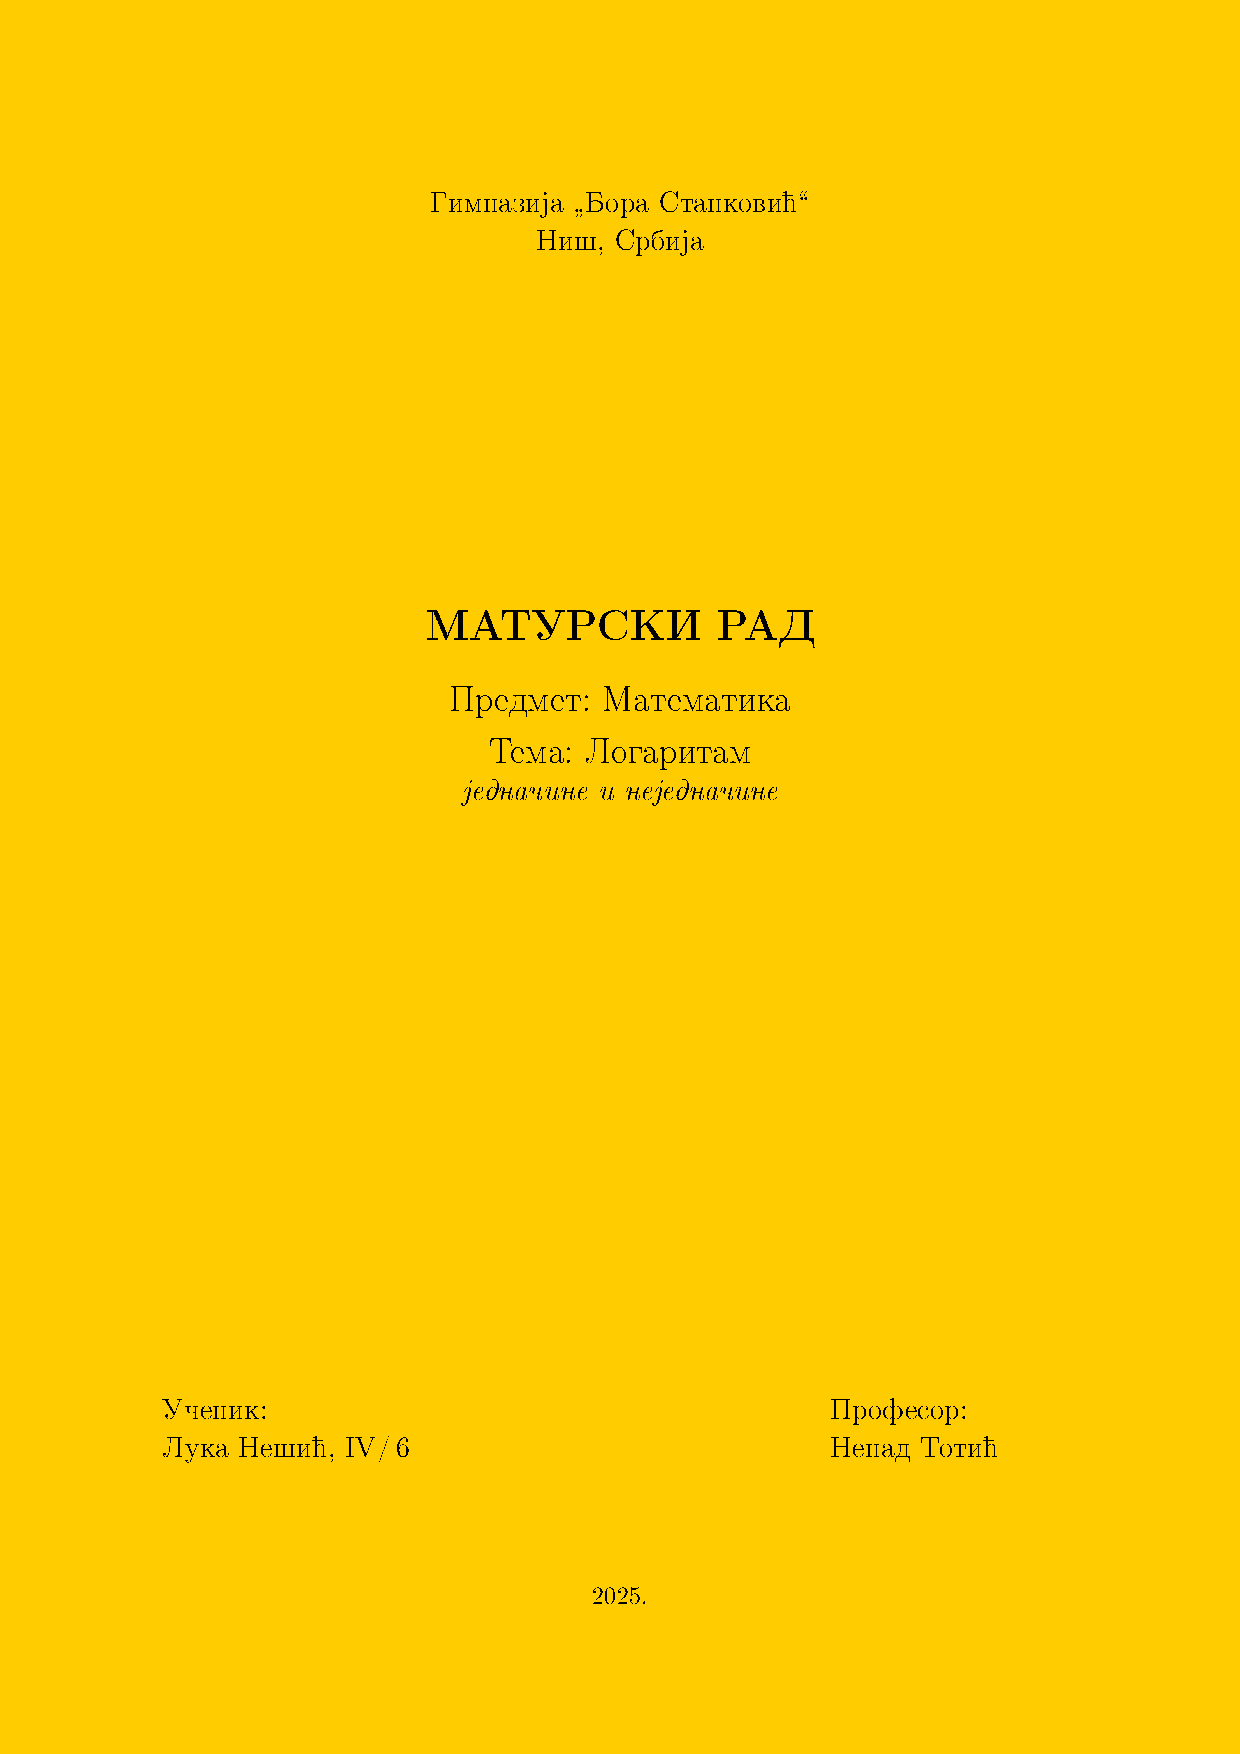
\includegraphics[]{log.2}}{Број $z$ у комплексној равни.}
$$
он може бити представљен као
\begin{alignat*}{3}\index{i@$i$}\index{поларни запис}
z 
&= x + iy &&\qquad\text{правоугле координате},\\
&= \rho\, (\cos\theta +i\sin\theta)&&\qquad\text{поларне координате}.
\end{alignat*}
Из Ојлерове формуле\index{Ојлерова формула}\footnote{Ојлерова формула
се лако доказује из формуле \eqref{eq:exp} и сличних формула
за $\sin x$ и $\cos x$, које се добијају из {\sl Меклореновог\index{Меклорен} реда\/}\index{Меклоренов ред}
(Cailean MacLabhruinn):
$f(x)=\sum_{n=0}^\infty\, f^{(n)}(0)\,(x^n/n!)$, где $f^{(n)}$ представља $n$-ти извод функције $f$.}
\begin{equation}\label{eq:euler}
  \okvir{\e^{i\theta} = \cos\theta + i\sin\theta},
\end{equation}
следи да је $z=\rho\,\e^{i\theta}$, одакле,
из једнакости \eqref{eq:lnmul} и \eqref{eq:powb} се добија\index{ln@$\ln$}
\begin{equation}\index{ln@$\ln$}
  \okvir{\ln z = \ln\rho + i\theta}.
  \label{eq:cln}
\end{equation}
Пошто је $\rho=|z|=\sqrt{x^2+y^2}\ge0$\index{апсолутна вредност $\vert x\vert$},
следи да природни логаритам комплексног броја $z$ није дефинисан само за $z=0$, када је
$\ln z=\rsinfty$.\index{комплексна бесконачност $(\rsinfty)$}
Како је $y/x=\tan\theta$, природни логаритам комплексног броја,
представљеног правоуглим координатама
може се израчунати
\begin{equation}
\okvir{\ln(x+iy)={\frac12}\ln(x^2+y^2)+i\arctan\left(\frac yx\right)},
\label{eq:clncart}
\end{equation}
као и
\begin{equation}\index{exp@$\exp$}
  \okvir{\exp(x+iy)=\e^x\,(\cos y+i\sin y)}.
  \label{eq:cexp}
\end{equation}


И за комплексне бројеве важи једнакост промене основе \eqref{eq:chgbase}, тако да за два комплексна броја
$z$ и $w$, где је $z\ne0$, $w\ne0$ и $w\ne1$, следи
$\log_w z=\ln z/\ln w$,
где се $\ln z$ и $\ln w$ рачунају помоћу формуле \eqref{eq:cln}, односно, \eqref{eq:clncart}.
На пример,
$$
\log_{2+i}(3+4i)=2, \qquad \log_i\e=\frac{2}{i\pi},\qquad \logtwo(-4)=2+\frac{i\pi}{\ln2}.
$$

Из Ојлерове формуле следи и
{\sl најлепша формула у историји математике},
у којој је употребљено 5 најважнијих математичких константи
($0,1,\pi,\e,i$)
\begin{equation}
  \okvir{\e^{i\pi}+1=0},
  \label{eq:zeuler}
\end{equation}
где, ако пребацимо 1 на десну страну и {\sl логаритмујемо}\index{логаритмовање}, добијамо једнакост
$$
\frac{\ln(-1)}{\sqrt{-1}}=\pi\index{пи $(\pi)$}.
$$

\input quaternions

\subsection{Извод}

Ако је
$$
y=\ln x\sledi y'=\frac1x,
$$
одакле се, помоћу једнакости \eqref{eq:chgbase} и једнакости за \idx{извод} сложене функције, добија
\begin{equation}
\okvir{y=\logb(f(x))\sledi y'=\frac{f'(x)}{f(x)\ln b}}.
\label{eq:izvod}
\end{equation}

\def\dx{{\it dx}}
\def\const{{\rm constant}}
\def\plusconst{{\color{gray}{}+\const}}
Површина фигуре испод функције
$y=1/x$ до $x$-осе\idxaxis x, у опсегу од 1~до~$x$ износи 
$\ln x$.
Математички записано: $\int_1^x\dx/x=\ln x$. 
$$
\slika{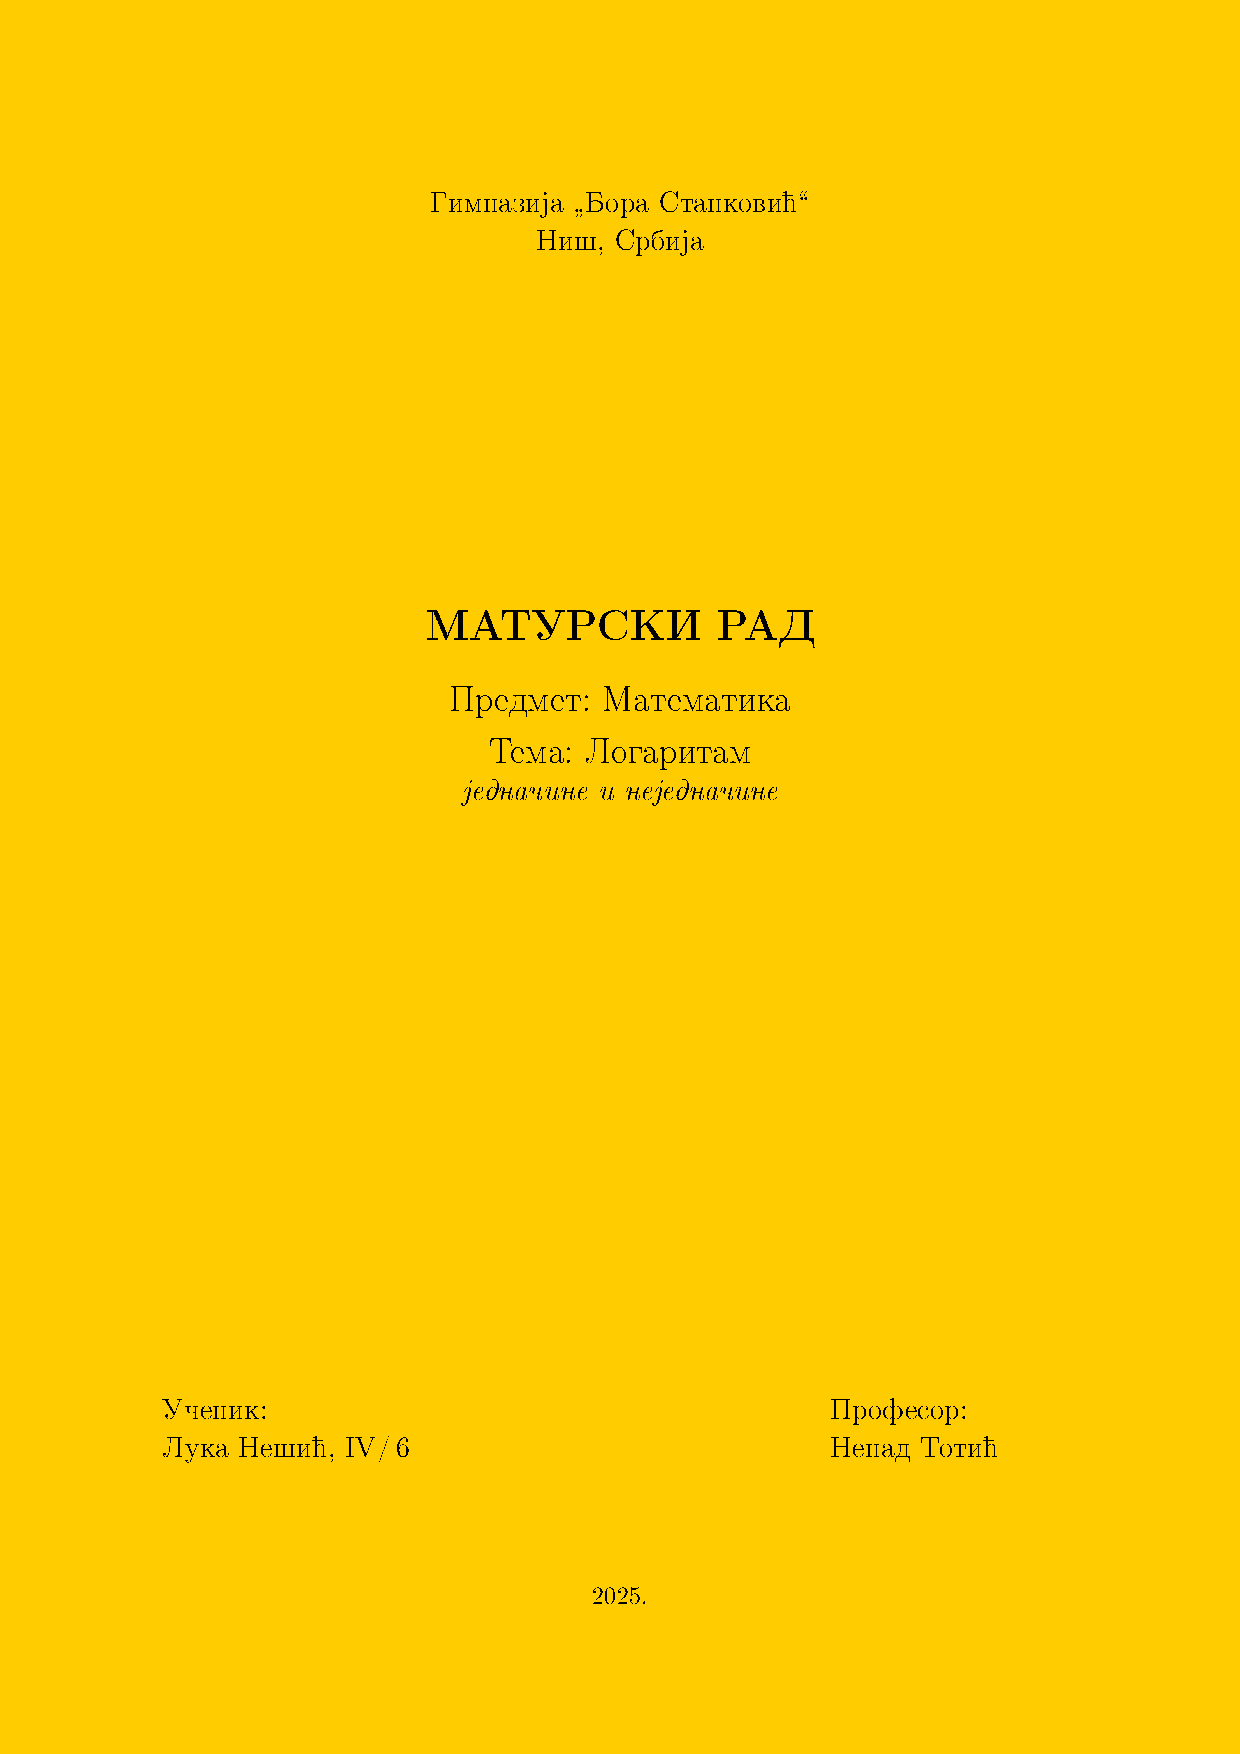
\includegraphics[]{log.3}}{Геометријско значење $\ln x$.\index{график}}
$$
(На слици је $x=\e$, тако да је површина осенчане фигуре једнака 1.)


\subsection{Интеграл}
Неодређени \idx{интеграл} природног логаритма је
\begin{equation}\label{eq:integral}
  \int \ln x\,\dx 
  = x \ln x - x \plusconst.
\end{equation}

\subsection{Лимес}\index{лимес}

\idx{Ојлер} је доказао да је
\begin{equation}\label{eq:limes}
  \ln x=\lim_{n\to\infty}n(\sqrt[n]x-1).
\end{equation}

\subsection{Бенфордов закон}

\def\fibonacci#1#2#3{%
\newcount\a \a=#1
\newcount\b \b=#2
\number\a,~\number\b
\newcount\t
\newcount\n \n=#3 \advance\n-3
\loop
  \t=\b \advance\b\a \a=\t
  , \number\b
  \advance\n-1\ifnum\n>0 
\repeat}

Вероватноћа да {\sl почетне цифре\/} неке математичке или физичке константе
(као и дужине реке, висине планине, броја становника, стања на рачуну, \dots), 
буду $\ell$ за бројну основу $b$, прати такозвани {\sl \idx{Бенфордов закон}\/} (Frank Benford), и износи
\begin{equation}\label{eq:benford}
  P(b,\ell)=\log_b \left(1+\frac1\ell\right).
\end{equation}

На пример, у {\sl Фибоначијевом низу\/}\index{Фибоначијев низ}: \fibonacci11{17},~\dots,
\idx{вероватноћа} да прва цифра неког члана низа буде $9$ износи $\logten(1+1/9)\approx4\.58\%$.
Ову законитост је открио 1881.\ године астроном \idx{Њуком} (Simon Newcomb), када је приметио да су
листови логаритамских таблица које је дуго користио најпрљавији на почетку:
\smash{\hbox{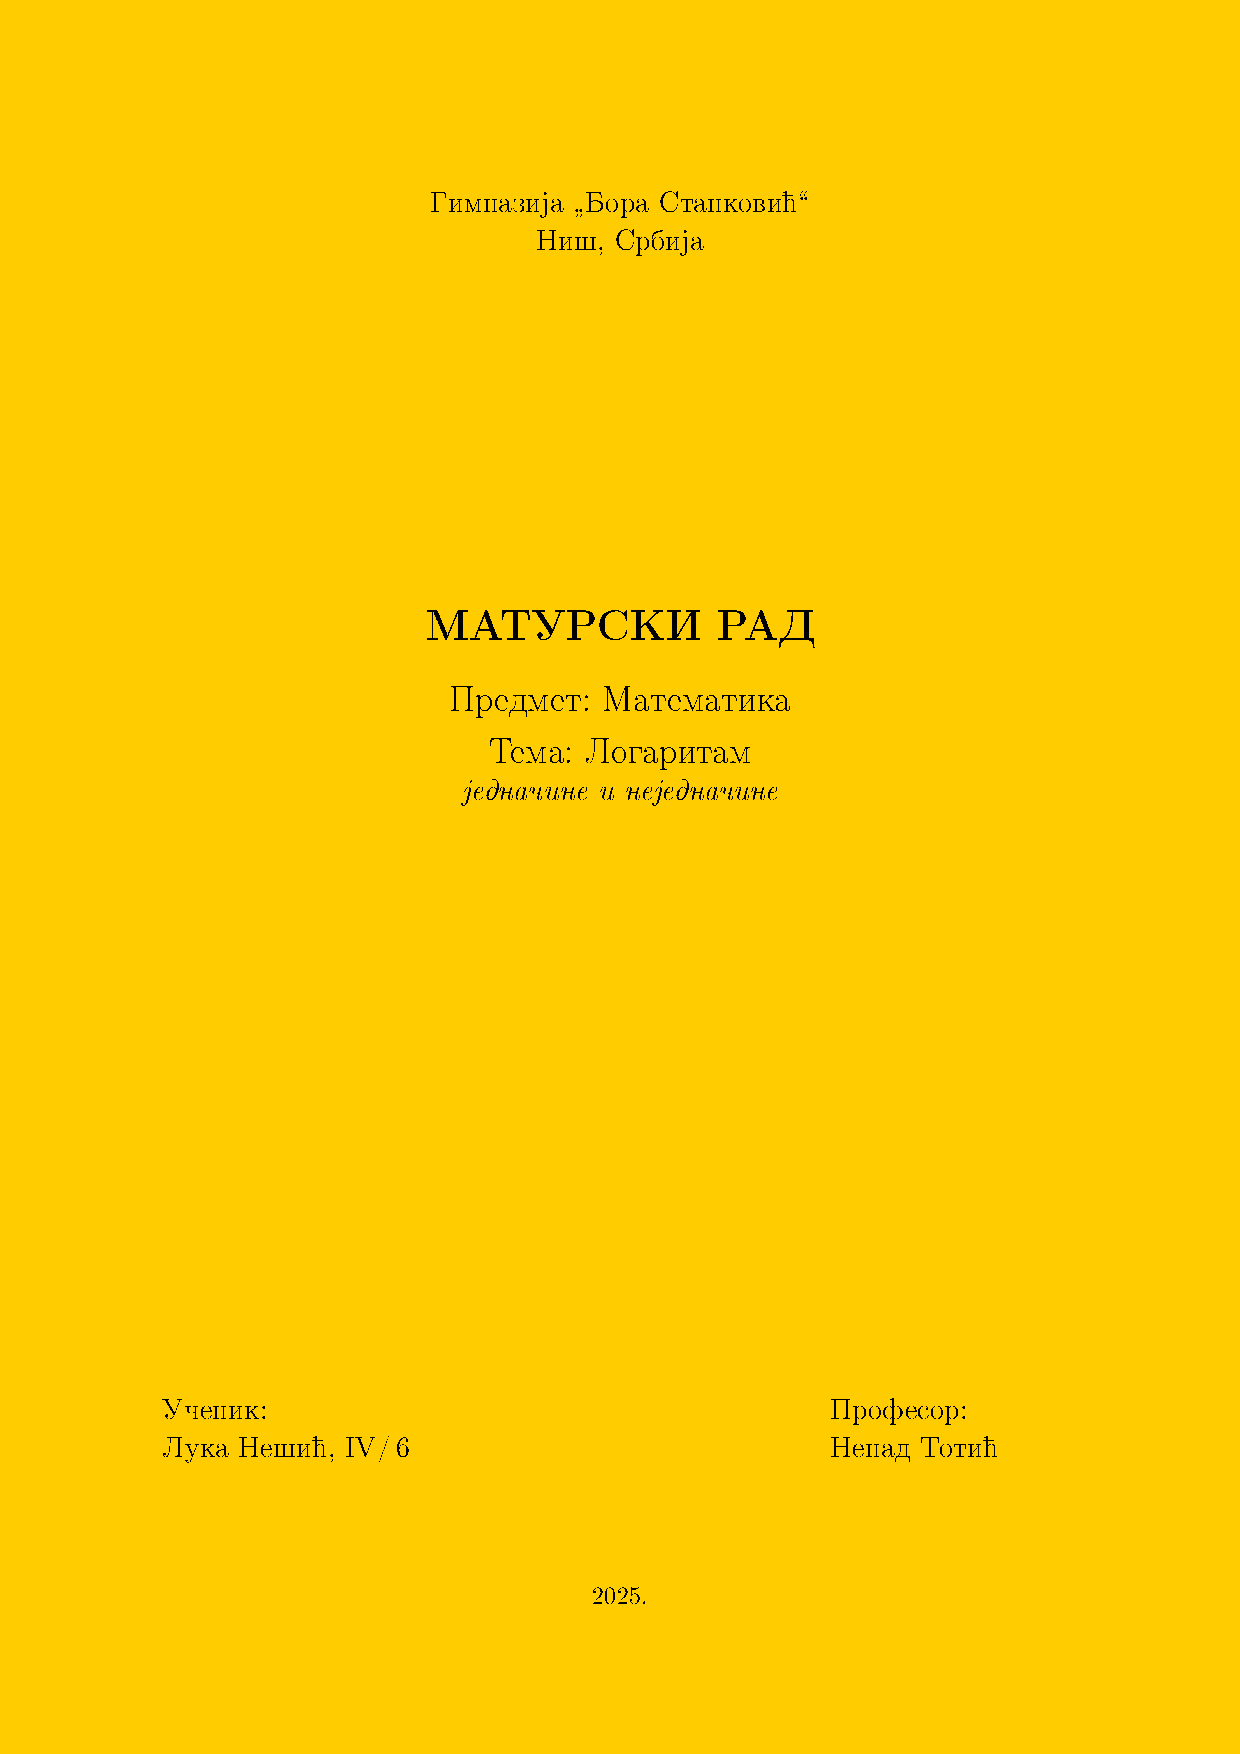
\includegraphics{log.4}}}.
(Видети задатак \ref{sssec:benford}.)

\newif\ifpnt \pntfalse
\ifpnt\input pnt\fi
